\subsection{\textit{Safespot}}
In 2006 a project running for 4 years called Safespot \cite{Safespot} was co-funded by the European Commission Information Society and Media, and had an objective to improve road safety. One of the key elements was to have vehicles exchange data between them and with infrastructure (\acrshort{V2V} and \acrshort{V2I}) to advice or warn the driver of upcoming situation happening.\par
% 
\subsubsection{Architecture}
Safespot is composed of nodes, that communicates with each other through short range wireless communication called \acrfull{VANET} using \hyperref[sec:802.11p]{IEEE 802.11p} as physical layer. A node can be in a vehicle or on an infrastructure such as a traffic light. All nodes create data through their sensors or through data from other nodes and are then collected in a multi-layered Database named \acrfull{LDM}.

\begin{figure}[h]
    \centering
    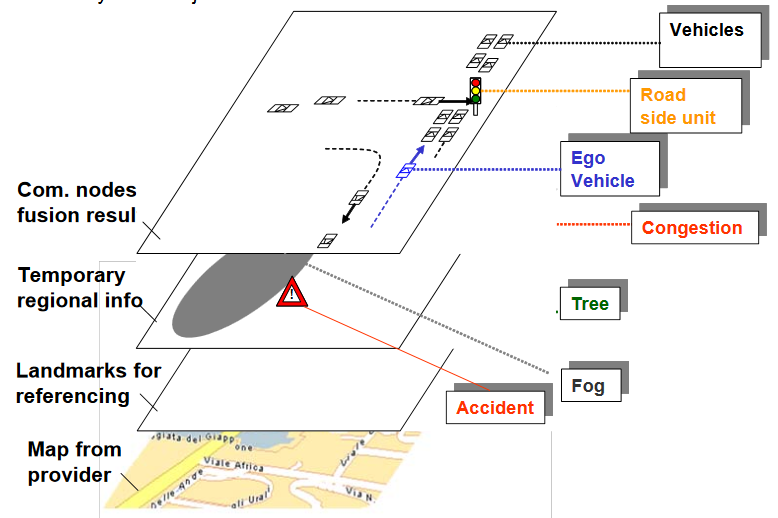
\includegraphics[width=14cm]{LDM-pic}
    \caption{Shows breakdown of \acrshort{LDM}. Taken from \url{http://www.safespot-eu.org/sp3.html}.}
    \label{fig:LDM}
\end{figure}

\acrshort{LDM} consist of 4 layers. From bottom up, the first is the static map like Google maps. The second is Landmarks, such as road signs, trees, buildings etc. The third is temporary objects that can change from day to day, such as road work. And lastly Dynamic object which is immediate status, such as congestion, current traffic light colour etc. \cite{Brignolo2008UseProject}.
To locate the position of the vehicles, Safespot uses the road data from \acrshort{GPS}, road landmark recognition and dead reckoning\footnotemark.\par
%
% 
\footnotetext{\textquote[Taken from: \url{https://en.wikipedia.org/wiki/Dead_reckoning}]{\textit{In navigation, dead reckoning or dead-reckoning is the process of calculating one's current position by using a previously determined position, or fix, and advancing that position based upon known or estimated speeds over elapsed time and course.}}}
% 
% 
The data rate and communication channel usage is restricted and is one of the physical bottle neck in the system. US \acrshort{wave} standard (which is similar to Safespot) has a specified data rate of:
\begin{itemize}[noitemsep]
    \item Remote \acrfull{OBU} (vehicle): 2320 bit/s
    \item Remote \acrlong{RSU} (traffic light): 22500 bit/s  
\end{itemize}
Though the numbers might be slightly different in Europe, it still shows the bottleneck that exists in this kind of communication channel, especially for \acrshort{OBU}s.\par
% 
Depending on how advanced we want the platooning to be, we could possibly lessen the amount of data transmitted and thus reduce the accuracy/latency/other parameters (within certain range). Since Safespot's main objective was safety, they needed as many details as possible, to make sure that the driver was given the correct information to avoid a incoming crash. If we want to make platooning only available on highways and only the speed and the brake being controlled, the amount of information needed to be sent to the \acrshort{VANET} is severely lessened, but if everything were to be automatised, at least as much data as Safespot is needed. The restriction of the data rate is something to take into consideration as well. 